% =============================================================================
% Paper B -- Target: Journal of Supercomputing / IEEE Transactions on Industrial Informatics
% =============================================================================
\documentclass[11pt,a4paper]{article}

\usepackage[utf8]{inputenc}
\usepackage[T1]{fontenc}
\usepackage{geometry}
\geometry{top=1in, bottom=1in, left=1in, right=1in}
\usepackage{amsmath}
\usepackage{amssymb}
\usepackage{microtype}
\usepackage{graphicx}
\usepackage{booktabs}
\usepackage{multirow}
\usepackage{xcolor}
\usepackage{hyperref}
\usepackage{cite}

\graphicspath{{figures/}}

\hypersetup{
    colorlinks=true,
    linkcolor=blue,
    filecolor=magenta,
    urlcolor=cyan,
    citecolor=blue,
}

\title{\textbf{Validated TensorRT Optimization of Self-Supervised Power-Converter Anomaly Detectors on Jetson Nano}}

\author{
    \textbf{Ignacio Martin-Salinas}, \textbf{Jose A. Belloch}, \textbf{Adri{\'a}n Amor-Mart{\'\i}n}, \\
    \textbf{Pablo Zumel}, \textbf{Cristina Fernandez} \\
    \small Department of Electronic Technology, Universidad Carlos III de Madrid \\
    \small 28911 Legan{\'e}s, Madrid, Spain
}
\date{}

\begin{document}
\maketitle

\begin{abstract}
Embedded inference for condition monitoring requires measuring execution cost and checking whether numerical optimization changes anomaly decisions. This paper presents a comprehensive systems-level optimization, cross-runtime benchmarking, and numerical fidelity evaluation of a self-supervised frequency-response anomaly detection pipeline on an NVIDIA Jetson Nano edge platform (Maxwell GPU, 128 CUDA cores, Quad-Core ARM Cortex-A57 CPU, 4~GB unified LPDDR4 memory, JetPack~4.6\,/\,TensorRT~8.2), an ultra-low-cost archetype for heterogeneous SoC performance methods. Under a strict batch-1 streaming protocol (15 warm-up iterations, 150 timed executions, monotonic host clock for CPU and CUDA events for GPU), we benchmark 60 attempted model--runtime--precision combinations (45 core FP32/FP16 configurations plus 15 INT8 configurations) spanning Keras, TensorFlow Lite, ONNX Runtime, and NVIDIA TensorRT across FP32, FP16, and INT8 precisions for five neural encoder architectures. To prevent aggressive quantization from distorting detector behavior, an anomaly-decision acceptance gate is enforced: paths exhibiting $>1\%$ decision discordance on the 1{,}268-sample held-out test set relative to the unquantized Keras FP32 baseline are marked as non-deployable. The core FP32/FP16 matrix yields 37 validated and 8 fidelity-rejected configurations; all 15 INT8 configurations are non-deployable (5 TensorRT engine-build failures and 10 CPU INT8 fidelity failures, see Sec.~\ref{sec:int8-exclusion}). No INT8 configuration is deployable on this target due to three compounding barriers: hardware absence of integer dot-product units in compute capability 5.3, TensorRT~8.2 ONNX parser rejection of per-channel QuantizeLinear/DequantizeLinear (QDQ) graphs, and CPU INT8 quantization noise that flips 49.8\%--54.6\% of threshold decisions. Among validated configurations, MLP in TensorFlow Lite FP32 attains the highest throughput and energy efficiency (0.168~ms latency, 710 sustained inferences/s, 6.33~mJ/inference). For recurrent architectures, TensorRT FP16 engine compilation resolves CPU execution bottlenecks with $43\times$ (GRU) and $52\times$ (LSTM) speedups while preserving fidelity, and serves as a performance-portability baseline for modern Ampere-class SoCs (Sec.~\ref{sec:discussion}).
\end{abstract}

\noindent\textbf{Keywords:} Edge Computing; TensorRT; Jetson Nano; Power Electronics; Anomaly Detection; Inference Validation; Embedded GPU; Post-Training Quantization

\section{Introduction}
\label{sec:intro}

Power electronic converters (PECs) are mission-critical components in aerospace power distribution, electric vehicle powertrains, and renewable energy grids, where undetected parametric component degradation can lead to catastrophic electrical failure~\cite{idrisov2025digitaltwin,liu2023review}. A companion methodological study~\cite{mmas_anomaly_detection} establishes a self-supervised contrastive autoencoder framework based on the CARLA principle~\cite{darban2025carla} that detects subtle parametric faults directly from converter frequency-domain transfer-function (Bode) signatures. 

While that companion study focuses on representation learning and physics-informed negative synthesis (the applied mathematical formulation), this paper addresses the complementary computer systems and performance-methods challenge central to \emph{The Journal of Supercomputing}: \emph{what is the exact computational, memory, power, and energy cost of executing these deep anomaly detectors in real time on heterogeneous, resource-constrained embedded hardware, and how do model architecture, numerical precision, and compiler lowering interact with accelerator runtimes?} The Jetson Nano exemplifies the heterogeneous SoC architecture (shared unified memory, no discrete VRAM, tightly coupled CPU--GPU) that increasingly characterizes edge supercomputing.

The target platform for this investigation is the NVIDIA Jetson Nano Developer Kit~\cite{nvidia2019jetsonnano}, representing an integrated System-on-Chip (SoC) combining a quad-core 64-bit ARM CPU with a 128-core Maxwell-architecture GPU sharing 4~GB of unified LPDDR4 memory. Prior investigations of deep learning for power electronics diagnostics have predominantly focused on diagnostic accuracy and self-commissioning algorithms~\cite{gomez2024selfcommissioning,beattie2022robust}, rarely addressing rigorous, cross-runtime latency, memory footprint, rail-level power consumption, and numerical fidelity on target embedded edge hardware. General deep learning benchmarking frameworks~\cite{banbury2021mlperftiny,baller2021deepedgebench,sze2017efficient} and quantization surveys~\cite{gholami2022quantsurvey,jacob2018quantization} provide benchmarking principles, but fail to address the \textbf{layer-level metric fallacy} inherent to one-class metric space anomaly detectors: proxy numerical errors (e.g., layer-wise MSE or cosine similarity) mask catastrophic downstream classification failures caused by low-precision truncation noise near decision boundaries.

The specific scientific and systems-level contributions of this paper are as follows:
\begin{enumerate}
    \item \textbf{Comprehensive Cross-Runtime Optimization Matrix:} We design and execute an optimization matrix spanning 60 attempted configurations (45 core FP32/FP16 plus 15 INT8) across Keras CPU~\cite{chollet2015keras}, Keras GPU~\cite{abadi2016tensorflow}, TensorFlow Lite (TFLite), ONNX Runtime~\cite{bai2019onnx}, and NVIDIA TensorRT~\cite{nvidia2020tensorrt} in FP32, FP16, and INT8 precisions across five encoder families (Section~\ref{sec:pipeline}). The deployable core of 45 FP32/FP16 configurations yields the 37/8 validated/rejected split; INT8 is systematically attempted but fully non-deployable (Sec.~\ref{sec:int8-exclusion}).
    \item \textbf{Downstream Anomaly-Decision Acceptance Criterion:} We establish an end-to-end numerical validation gate that replaces proxy tensor MSE with final thresholded classification concordance across 1,268 held-out test states, exposing that uncalibrated low-precision integer paths flip nearly half of all safety-critical diagnostic decisions (Section~\ref{sec:methodology}).
    \item \textbf{Decoupled Single-Sample Timing and Latency Budgeting:} We formulate a single-sample ($n=1$) streaming evaluation protocol incorporating 15 discarded warm-up iterations and 150 timed executions, decomposing total detector latency into preprocessing, neural inference, and reference-bank metric evaluation (Section~\ref{sec:methodology}).
    \item \textbf{Physical Hardware Profiling and Rail Energy Measurement:} We conduct multi-repetition hardware campaigns on the Jetson Nano to capture active/idle system shared RAM, process resident set size (RSS), CUDA driver memory allocation, CPU/GPU utilization, thermal profiles, and continuous 10-Hz INA3221 rail power consumption via the PMLib framework, formally separating dynamic workload energy from carrier quiescent power (Section~\ref{sec:results-edge}).
    \item \textbf{Vertical Root-Cause Diagnosis of Quantization Breakdown:} We provide a cross-stack diagnosis spanning Silicon ISA limitations (Compute Capability 5.3 lacking hardware integer acceleration), Compiler IR lowering (TensorRT 8.2 QDQ parser rejections), and metric space boundary perturbations (Section~\ref{sec:pipeline}).
\end{enumerate}

\section{Related Work}
\label{sec:related}

\subsection{Quantization and Efficient Neural Inference}
Post-Training Quantization (PTQ) reduces the memory bandwidth, computational latency, and energy footprint of deep neural networks by mapping 32-bit floating-point parameters and activations to 16-bit float or 8-bit integer representations~\cite{sze2017efficient,jacob2018quantization,gholami2022quantsurvey}. PTQ literature demonstrates that bit-width allocation, symmetric versus asymmetric scaling, and calibration dataset selection heavily dictate accuracy preservation~\cite{latotzke2022posttraining}. Importantly, Latotzke et al.~\cite{latotzke2022posttraining} showed that intermediate layer-level MSE is an unreliable proxy for downstream task performance. In this study, we demonstrate that this disconnect is especially severe in one-class anomaly detection: because nominal test scores cluster near the calibrated anomaly threshold, minor rounding errors in reduced-precision latent spaces induce widespread classification decision flips.

\subsection{Embedded and Edge AI Benchmarking}
Standardized benchmarking suites such as MLPerf Tiny~\cite{banbury2021mlperftiny} establish rigorous timing and energy measurement protocols for microcontroller- and SoC-class edge hardware. DeepEdgeBench~\cite{baller2021deepedgebench} extends these principles across diverse embedded platforms, showing that the optimal runtime framework is highly model- and hardware-dependent. This study applies a comparable benchmarking rigor to power converter anomaly detection, integrating single-sample execution timing, unified memory decomposition, and physical INA3221 power rail telemetry.

\subsection{Embedded GPU Inference and Architecture Nuances}
NVIDIA Jetson-class SoCs integrate multi-core ARM CPUs with CUDA-capable GPUs sharing a unified LPDDR4 physical memory bus. This architecture makes memory allocation, PCIe-free zero-copy transfers, and thermal throttling interdependent design variables~\cite{swaminathan2024benchmarking}. On the Jetson Nano, prior studies have investigated model compression and knowledge distillation for out-of-distribution detection~\cite{bansal2024compressing} and highlighted the performance sensitivity of TensorRT graph compilation~\cite{swaminathan2024benchmarking}. Furthermore, multi-accelerator research emphasizes that precision-aware hardware mapping must jointly optimize accuracy, latency, and power~\cite{risso2024precisionaware}.

\subsection{Edge Diagnostics in Power Electronics}
Data-driven condition monitoring for power converters increasingly targets embedded microcontrollers and edge SoCs to enable real-time local protection~\cite{gomez2024selfcommissioning,idrisov2025digitaltwin,beattie2022robust}. However, existing literature largely focuses on algorithmic design without reporting physical rail energy consumption, operator lowering coverage, or numerical verification on target edge hardware.

\section{Workload Background: Anomaly Detection Pipeline}
\label{sec:background}

The workload evaluated in this benchmark is the self-supervised anomaly detection pipeline detailed in the companion study~\cite{mmas_anomaly_detection}. The input signature represents the small-signal duty-cycle-to-output-voltage frequency response $G_{vd}(s)$ of a synchronous buck converter plant, evaluated at $N_f = 101$ logarithmically spaced frequencies from $100\text{ Hz}$ to $50\text{ kHz}$. Magnitude and phase responses are converted to standardized real and imaginary channels, yielding an input tensor $\mathbf{X} \in \mathbb{R}^{101 \times 2}$.

The model consists of an encoder backbone $f_{\boldsymbol{\theta}}(\cdot)$ coupled with a multi-layer projection head $g_{\boldsymbol{\phi}}(\cdot)$ producing an $L_2$-normalized latent embedding $\mathbf{z} \in \mathbb{R}^{d_{\mathrm{proj}}}$. Five distinct encoder backbones are evaluated:
\begin{enumerate}
    \item \textbf{Conv1D-AE:} 1-D strided convolutional layers capturing local frequency correlations.
    \item \textbf{GRU-AE:} Bidirectional Gated Recurrent Units with linear-before-reset semantics.
    \item \textbf{LSTM-AE:} Bidirectional Long Short-Term Memory recurrent cells.
    \item \textbf{MLP-AE:} Multi-Layer Perceptron dense feedforward baseline.
    \item \textbf{Transformer-AE:} Multi-Head Self-Attention sequence architecture.
\end{enumerate}

Each exported embedding is evaluated using its fitted reference detector. LSTM uses Euclidean $k$-nearest-neighbor distance with $k=1$ against the 2,419 healthy training embeddings. Conv1D, GRU, MLP, and Transformer use regularized Mahalanobis distance fitted to healthy training embeddings. The scorer and healthy-score percentile were selected by F1 on the labeled fit-validation split. The selected percentile is 98 for Conv1D and 95 for the remaining models. The persisted test split comprises 1,268 states (520 healthy and 748 anomalous) for downstream fidelity evaluation.

\section{Model Optimization Pipeline and Lowering Paths}
\label{sec:pipeline}

Table~\ref{tab:formats} outlines the deployment runtimes, formats, and precisions evaluated on the Jetson Nano. We attempt 60 combinations (12 per architecture: 1 Keras Native FP32 $+$ 2 Keras GPU $+$ 3 TFLite $+$ 3 ONNX $+$ 3 TensorRT); the 45 core FP32/FP16 combinations form the validated/rejected matrix, while 15 INT8 combinations are non-deployable (Sec.~\ref{sec:int8-exclusion}). Every format is evaluated with a \textbf{fixed batch size of one} ($n=1$), matching the streaming, sample-by-sample execution required in real-time converter supervisory systems.

\begin{table}[t]
\centering
\caption{Evaluated deployment runtimes, lowering pathways, and precisions.}
\label{tab:formats}
\resizebox{\textwidth}{!}{%
\begin{tabular}{@{}llll@{}}
\toprule
Runtime Backend & Model Format & Evaluated Precisions & Target Hardware \\
\midrule
Keras Native & Native SavedModel & FP32 (Baseline) & Nano ARM CPU \\
Keras GPU & TensorFlow Graph Engine & FP32, Mixed FP16 & Nano Maxwell GPU \\
TensorFlow Lite & FlatBuffer & FP32, Float16 PTQ, Integer PTQ (INT8) & Nano ARM CPU \\
ONNX Runtime & Graph Proto & FP32, FP16 PTQ, Static QDQ (INT8) & Nano ARM CPU \\
NVIDIA TensorRT & Serialized Plan & FP32, FP16 Engine, QDQ Engine (INT8) & Nano Maxwell GPU \\
\bottomrule
\end{tabular}%
}
\end{table}

\subsection{Model Conversion and Graph Lowering}
Training is executed on a workstation NVIDIA RTX~4070 GPU. Following training, checkpoint weights, reference banks, and preprocessing scalers are transferred to the Jetson Nano. All framework-neutral ONNX serialization~\cite{bai2019onnx}, TFLite conversion, FP16 reduction, QDQ calibration, and TensorRT engine compilation~\cite{nvidia2020tensorrt} are performed natively within the JetPack 4.6 software stack~\cite{nvidiajetpackarchive} on the Jetson Nano.

Post-Training Quantization (PTQ)~\cite{tensorflowliteptq,onnxruntimequantization} utilizes a fixed calibration dataset of 100 representative samples drawn from the healthy training partition, with exact SHA-256 tensor verification. For TensorFlow Lite, full-integer PTQ applies representative dataset calibration to restrict internal kernel execution to 8-bit integers while preserving FP32 input/output bindings. ONNX INT8 quantization generates explicit QuantizeLinear/DequantizeLinear (QDQ) operator pairs with symmetric per-tensor activation scaling and symmetric per-channel weight scaling.

\subsection{Recurrent Operator Lowering (GRU and LSTM)}
For recurrent architectures, TensorRT~8.2 supports native recurrent layers through its internal RNNv2 interface~\cite{nvidia2022tensorrt825}. The exporter maps trained Keras input kernels, recurrent kernels, and bias vectors directly to ONNX GRU and LSTM operator nodes. LSTM gate tensors are mapped from Keras $[i,f,c,o]$ ordering to ONNX $[i,o,f,c]$ conventions. For GRU, separate input and recurrent bias vectors are preserved to maintain linear-before-reset mathematical equivalence. Each exported graph is validated through ONNX Runtime on CPU before submission to the TensorRT ONNX parser.

\subsection{Transformer Graph Rewriting}
The Transformer-AE architecture is exported to ONNX by expressing multi-head attention via explicit rank-3 batched matrix multiplications and numerically stable softmax normalization $\mathrm{Softmax}(\mathbf{S}) = \exp(\mathbf{S} - \max \mathbf{S}) / \sum \exp(\mathbf{S} - \max \mathbf{S})$. The resulting computational graph undergoes exact projection MSE verification against the Keras reference before TensorRT plan compilation.

\subsection{Systematic Analysis of INT8 Exclusion}
\label{sec:int8-exclusion}
Calibrated INT8 execution was attempted for every architecture across all runtimes (15 INT8 configurations: 5 TFLite INT8 $+$ 5 ONNX INT8 $+$ 5 TensorRT INT8). However, no INT8 configuration is deployable, due to three independent failure mechanisms:
\begin{enumerate}
    \item \textbf{Hardware Architecture Incompatibility:} Fast INT8 execution in TensorRT relies on dedicated hardware integer dot-product instructions (e.g., DP4A on Pascal CC 6.1+ or Tensor Cores on Volta/Turing CC 7.0+). The Jetson Nano's Tegra X1 Maxwell GPU (compute capability 5.3) possesses no integer acceleration hardware~\cite{nvidia2021tensorrt82matrix}. The native TensorRT builder explicitly reports lack of native fast INT8 hardware execution support (Table~\ref{tab:hardware}).
    \item \textbf{Parser and Importer Rejection:} TensorRT~8.2 imports quantized ONNX graphs strictly as QDQ pairs around supported compute operators and rejects pre-quantized INT8 weights on scaling or batch-normalization nodes~\cite{nvidia2021tensorrt82guide}. On the Jetson Nano, every INT8 engine build fails during graph import, either halting with invalid INT8 weight type errors on batch-normalization and dense scaling operands (Conv1D, MLP, Transformer) or raising unsupported constant-operand exceptions on recurrent nodes (GRU, LSTM), triggering parser crashes. Restricting QDQ pairs exclusively to compute kernels (Conv, Gemm) reproduces the identical parser crash.
    \item \textbf{Downstream Decision Invalidation on CPU:} On the ARM CPU, all ten calibrated INT8 paths (TFLite INT8 and ONNX INT8) execute successfully and exhibit the highest raw throughputs (up to 825.98 inf./s for MLP). However, evaluated on the 1,268-sample test set, CPU INT8 alters \textbf{49.8\% to 54.6\%} of all threshold classification decisions relative to the baseline detector. Because one-class anomaly detectors operate on tightly clustered nominal distributions, minor integer truncation errors shift projection distances across the calibrated threshold $\gamma$, destroying classification validity.
\end{enumerate}

\section{Edge Hardware Testbed: Heterogeneous SoC Architecture}
\label{sec:hardware}

\begin{table}[t]
\centering
\caption{NVIDIA Jetson Nano edge benchmarking testbed specification.}
\label{tab:hardware}
\begin{tabular}{@{}lp{0.73\textwidth}@{}}
\toprule
Subsystem & Configuration Specification \\
\midrule
CPU & Quad-core ARM Cortex-A57 @ 1.43 GHz (64-bit) \\
GPU & 128-core NVIDIA Maxwell GPU @ 921 MHz (Compute Capability 5.3)~\cite{nvidia2019jetsonnano} \\
Memory & 4 GB 64-bit LPDDR4 @ 1600 MHz (25.6 GB/s shared unified memory) \\
Storage & 64 GB UHS-I microSD Class 10 \\
Operating System & Linux for Tegra (L4T 32.7.6, Ubuntu 18.04 LTS) \\
Toolchain Stack & JetPack 4.6.6~\cite{nvidiajetpackarchive}; CUDA 10.2; cuDNN 8.2.1; TensorRT 8.2.1.8 \\
Power Mode & MAXN (10 W unconstrained power budget; CPU/GPU/EMC clocks fixed) \\
Power Telemetry & Texas Instruments INA3221 3-channel power monitor sampled via PMLib~\cite{barrachina2013integrated} \\
\bottomrule
\end{tabular}
\end{table}

All edge benchmarks are executed physically on the Jetson Nano testbed described in Table~\ref{tab:hardware}. Operating clocks are locked at maximum frequency using system clock locking utilities to eliminate dynamic voltage and frequency scaling (DVFS) variance. Workload power is measured directly from the physical INA3221 sensor rails.

\section{Benchmarking Methodology: Performance Methods}
\label{sec:methodology}

\textbf{Unified Timing and Latency Protocol.} Every runtime backend executes single-sample streaming inference ($n=1$) using 15 discarded warm-up iterations followed by 150 consecutive timed runs. Host CPU executions are timed using high-resolution monotonic host clock timers. GPU executions in TensorRT are timed via CUDA events recorded on the dedicated execution stream. For Keras GPU, device synchronization barriers bracket the forward model call to ensure asynchronous kernels complete within the measured interval.

The complete detector latency includes spectral preprocessing and data movement, neural forward execution, and model-specific scoring and thresholding. The latency tables report measured neural forward times. The projection dimension is 512 for Conv1D, LSTM, and MLP, 256 for GRU, and 128 for Transformer. The runtime-fidelity comparison applies the corresponding reference detector to the embeddings from each backend. End-to-end latency requires a separate measurement of acquisition, preprocessing, and scoring on the target.

\textbf{Unified Memory Characterization.} Because CPU and GPU share physical LPDDR4 memory, discrete VRAM is not physically meaningful. We record three non-additive memory metrics:
\begin{enumerate}
    \item \textbf{System Shared RAM Peak $\Delta$:} Total system memory consumption relative to pre-load idle baseline, sampled at 100~ms via system performance telemetry.
    \item \textbf{Process RSS Peak $\Delta$:} Resident Set Size growth from process status telemetry.
    \item \textbf{CUDA Memory Allocation Peak $\Delta$:} Device memory allocated by the active CUDA context, queried via CUDA runtime driver memory interfaces.
\end{enumerate}

\textbf{Numerical Acceptance and Fidelity Gate.} Every optimized format is evaluated across the complete 1,268 held-out test states. We compute: (1) projection embedding MSE relative to Keras FP32, (2) continuous anomaly score correlation, and (3) threshold decision discordance percentage. A model format is marked \textbf{fidelity-rejected} if its full-test decision discordance exceeds 1.0\%.

\textbf{Power and Energy Measurement Protocol.} Resource profiling runs in three independent fresh processes per configuration, separated by 5-s thermal cooldown intervals. In parallel with 100-ms system telemetry monitoring, the PMLib framework~\cite{barrachina2013integrated} samples the on-board INA3221 monitor at 10 Hz across a 5-s idle window ($P_{\mathrm{idle,IN}} \approx 2.43\text{ W} \pm 0.02\text{ W}$) and a 15-s sustained inference window ($P_{\mathrm{active,IN}}$). We monitor total module input power, GPU rail power, and CPU rail power. We divide the mean module input power by sustained throughput to estimate total energy per inference. For dynamic energy we first subtract the mean idle input power. With power in watts and throughput in inferences per second, the factor of $10^3$ expresses the estimates in millijoules per inference.
\begin{align}
E_{\mathrm{total}} &= 10^3\frac{P_{\mathrm{active,IN}}}{q}\,, \\
E_{\mathrm{dynamic}} &= 10^3\frac{P_{\mathrm{active,IN}}-P_{\mathrm{idle,IN}}}{q}\,,
\label{eq:energy-def}
\end{align}
where $q$ denotes sustained throughput.

\section{Results and Performance Analysis}
\label{sec:results-edge}

\begin{figure}[t]
\centering
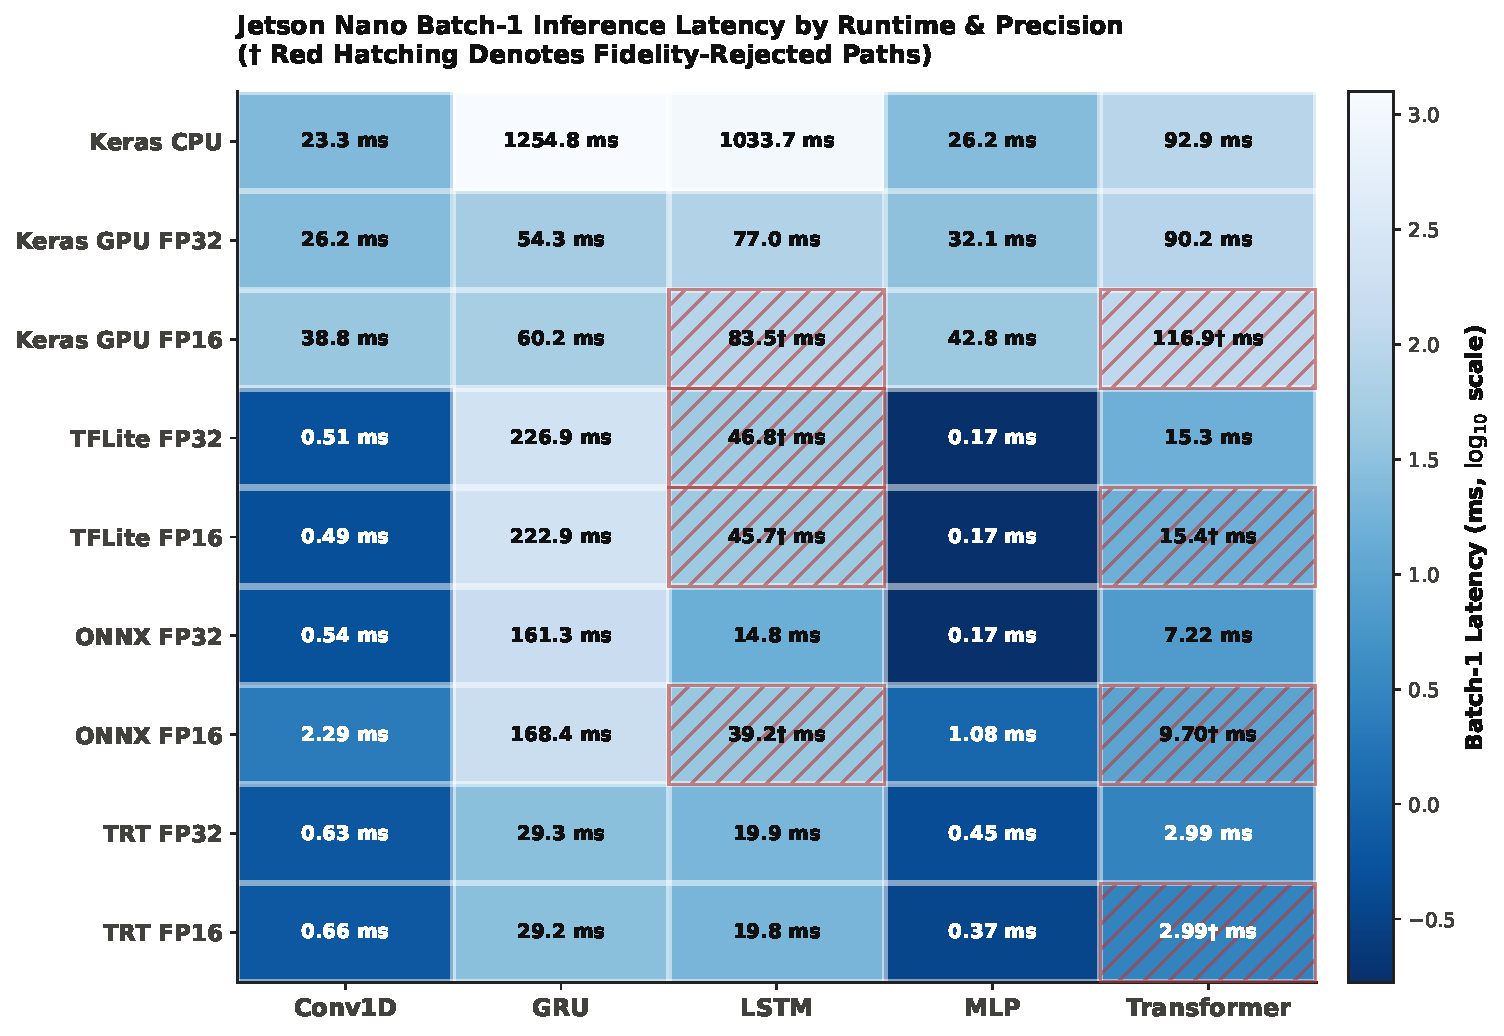
\includegraphics[width=0.98\textwidth]{jetson_precision_matrix.pdf}
\caption{Measured batch-1 inference latency across the 45 core FP32/FP16 model--runtime--precision combinations on NVIDIA Jetson Nano (60 attempted including 15 non-deployable INT8 configurations, Sec.~\ref{sec:int8-exclusion}).}
\label{fig:precision-matrix}
\end{figure}

\begin{figure}[t]
\centering
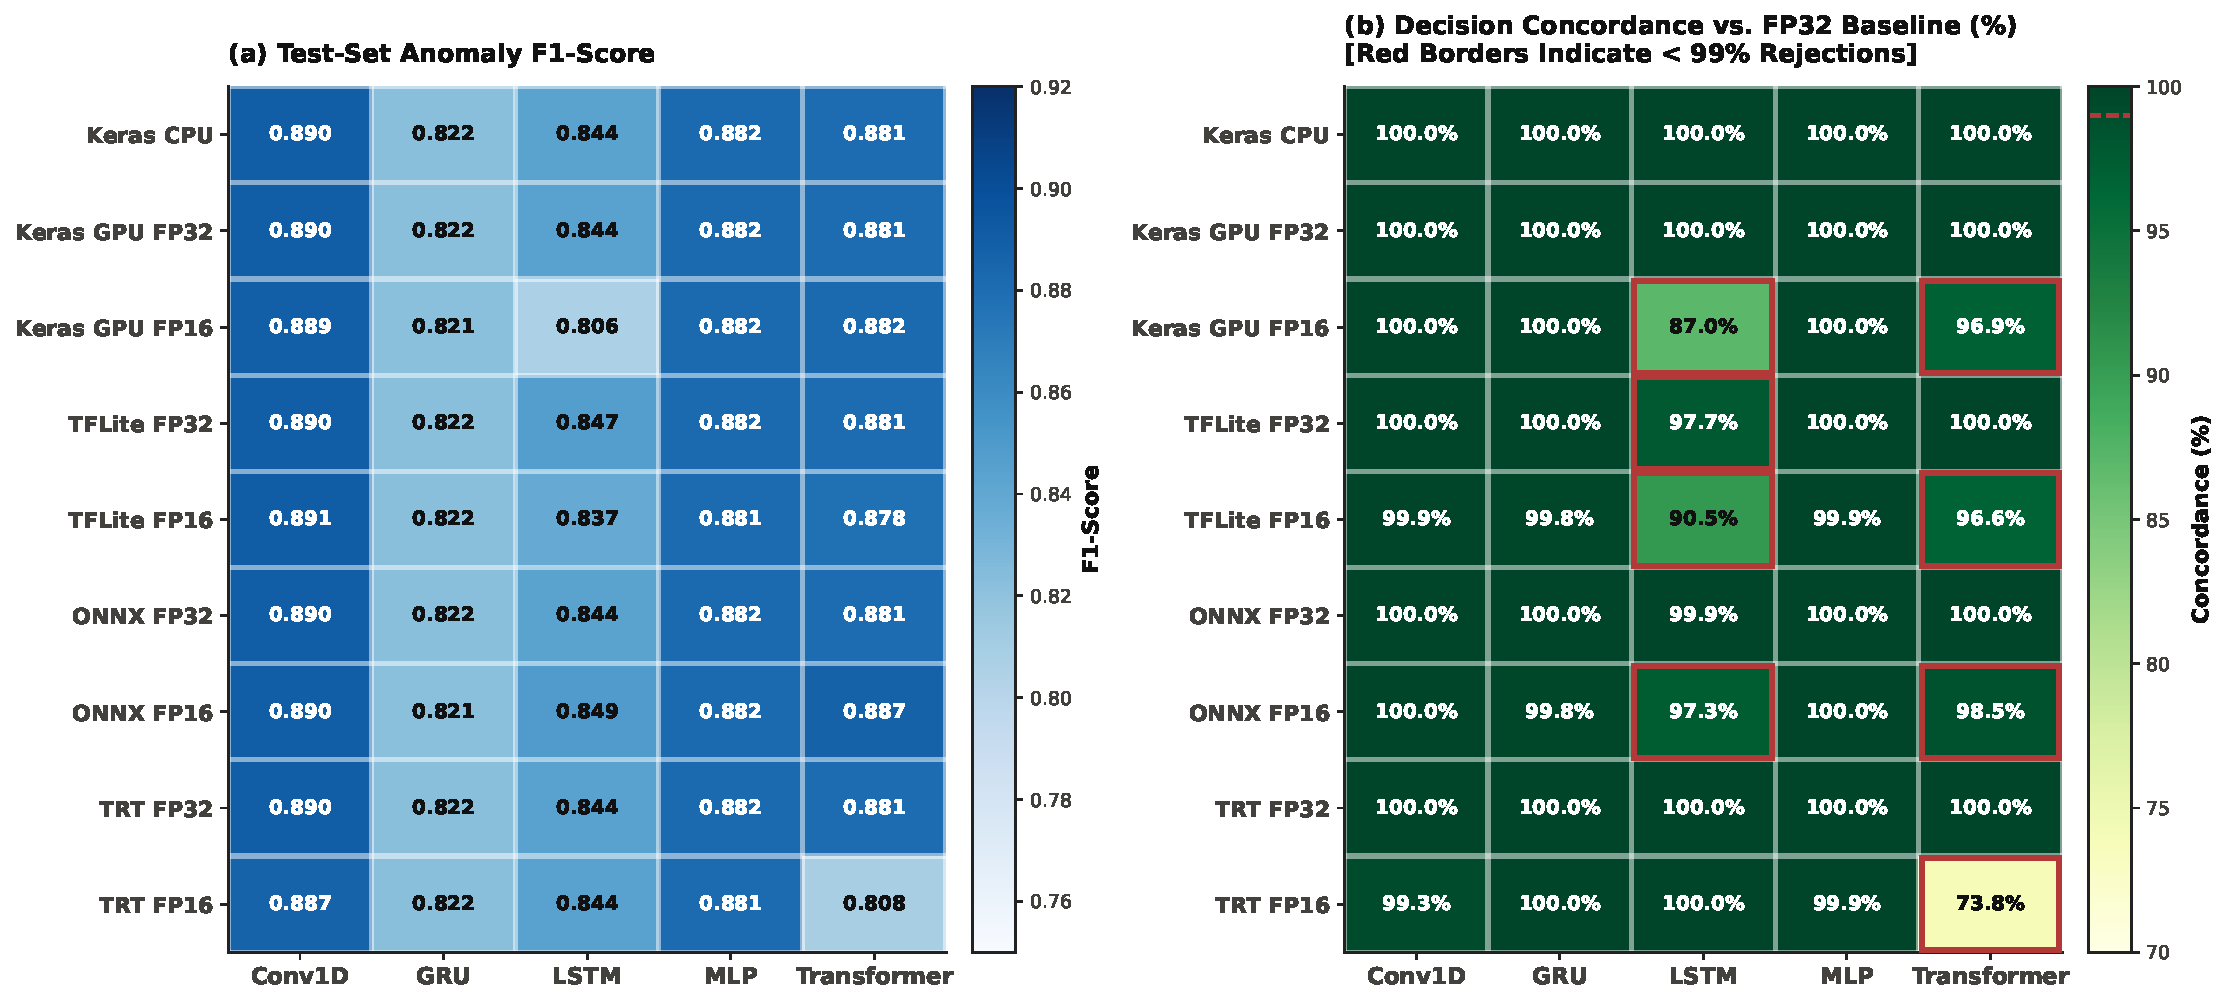
\includegraphics[width=0.98\textwidth]{jetson_optimization_fidelity.pdf}
\caption{Inference validation and numerical fidelity across optimization runtimes: (a) test-set anomaly detection F1-score; (b) anomaly decision concordance relative to Keras FP32 baseline (\%). Paths with $<99\%$ concordance are marked as fidelity-rejected.}
\label{fig:optimization-fidelity}
\end{figure}

\begin{table}[t]
\centering
\small
\caption{Numerical validation status across the core FP32/FP16 precision matrix (45 combos). V: Validated ($\le 1\%$ decision discordance); R: Fidelity-Rejected ($> 1\%$). INT8 (15 combos: 5 TFLite $+$ 5 ONNX $+$ 5 TensorRT) is fully non-deployable (Sec.~\ref{sec:int8-exclusion}). Including the two Keras GPU FP16 rejections not shown here, the core matrix contributes 8 fidelity rejections total (37 validated, 8 rejected).}
\label{tab:precision-status-core}
\label{tab:precision-status}
\begin{tabular}{@{}lcccccc@{}}
\toprule
 & \multicolumn{2}{c}{TensorFlow Lite} & \multicolumn{2}{c}{ONNX Runtime} & \multicolumn{2}{c}{NVIDIA TensorRT} \\
Model Architecture & FP32 & FP16 & FP32 & FP16 & FP32 & FP16 \\
\midrule
Conv1D-AE      & V & V & V & V & V & V \\
GRU-AE         & V & V & V & V & V & V \\
LSTM-AE        & R & R & V & R & V & V \\
MLP-AE         & V & V & V & V & V & V \\
Transformer-AE & V & R & V & R & V & R \\
\bottomrule
\end{tabular}
\end{table}

Fig.~\ref{fig:precision-matrix} illustrates the batch-1 execution latency across the 45 core FP32/FP16 configurations (60 attempted with INT8), while Fig.~\ref{fig:optimization-fidelity} and Table~\ref{tab:precision-status} (core matrix) report the corresponding F1-score preservation and decision concordance percentages.

\subsection{Numerical Fidelity Analysis}
Auditing weights, preprocessor parameters, and reference embeddings confirms byte-level equivalence between workstation and edge environments. Decision discordance varies across runtime conversions and numerical precisions:
\begin{itemize}
    \item \textbf{LSTM Conversion Fragility:} LSTM is the most fragile architecture under standard CPU conversions. TFLite FP32 and FP16 discard 2.3\% and 9.5\% of decisions, ONNX FP16 discords on 2.7\%, and native Keras GPU mixed FP16 discords on 13.0\%. Among the exported LSTM paths, ONNX FP32 and both TensorRT precisions meet the acceptance threshold.
    \item \textbf{Transformer Precision Sensitivity:} Transformer-AE fails reduced-precision validation across all backends: TFLite FP16 discords on 3.4\%, ONNX FP16 on 1.5\%, native GPU mixed FP16 on 3.1\%, and TensorRT FP16 alters 26.2\% of decisions. Only its FP32 paths achieve full validation (zero observed discordance).
    \item \textbf{Validated Baselines:} Conv1D, GRU, and MLP validate successfully across all FP32 and FP16 runtimes, maintaining decision discordances below 0.71\%.
\end{itemize}

\begin{table}[p]
\centering
\scriptsize
\setlength{\tabcolsep}{2.5pt}
\caption{Comprehensive batch-1 execution metrics on NVIDIA Jetson Nano (organized by model and hardware target). Evaluation latency reflects 150 timed runs of the core neural model (monotonic clock for CPU, CUDA events for GPU); throughput, memory, utilization, temperature, power and energy represent mean values over three isolated 15-s profiling repetitions. System RAM $\Delta$ and Process RSS $\Delta$ are host-measured; CUDA Mem $\Delta$ is device allocation (--- for CPU-only runtimes). Total energy uses active module input power. Dynamic energy subtracts idle input power ($P_{\mathrm{idle,IN}}\approx2.43$~W) before dividing by throughput. A dagger ($^\dagger$) denotes fidelity-rejected ($>1\%$ decision discordance). INT8 configurations are discussed separately in Sec.~\ref{sec:int8-exclusion}.}
\label{tab:selected-results}
\resizebox{\textwidth}{!}{%
\begin{tabular}{@{}l l r r r r r r r r r r r@{}}
\toprule
Model & Runtime Backend & Latency & Throughput & Sys.\ RAM $\Delta$ & RSS $\Delta$ & CUDA $\Delta$ & CPU & GPU & Temp & Active Power & $E_{\mathrm{total}}$ & $E_{\mathrm{dynamic}}$ \\
 & & (ms) & (inf./s) & (MB) & (MB) & (MB) & (\%) & (\%) & ($^\circ$C) & (W) & (mJ/inf.) & (mJ/inf.) \\
\midrule
\multirow{9}{*}{Conv1D} & Keras CPU & 23.308 & 39.13 & 225.5 & 372 & --- & 98.9 & 0.0 & 47 & 4.14 & 106.0 & 43.95 \\
 & TFLite FP32 & 0.513 & 541.18 & 200.6 & 342 & --- & 99.2 & 0.0 & 47 & 4.59 & 8.47 & 3.93 \\
 & TFLite FP16 & 0.492 & 541.88 & 204.7 & 345 & --- & 99.1 & 0.0 & 47 & 4.56 & 8.41 & 3.93 \\
 & ONNX FP32 & 0.544 & 139.31 & 211.7 & 361 & --- & 99.2 & 0.0 & 47 & 4.32 & 31.10 & 13.64 \\
 & ONNX FP16 & 2.289 & 103.80 & 207.6 & 356 & --- & 99.1 & 0.0 & 47 & 4.37 & 42.13 & 18.64 \\
 & TensorRT FP32 & 0.634 & 360.51 & 1103.7 & 1644 & 1388 & 97.9 & 7.7 & 47 & 4.87 & 13.50 & 6.76 \\
 & TensorRT FP16 & 0.658 & 363.08 & 1098.5 & 1647 & 1099 & 97.9 & 6.9 & 48 & 4.84 & 13.36 & 6.68 \\
 & Keras GPU FP32 & 26.173 & 33.31 & 2020.9 & 1931 & 1626 & 96.6 & 1.6 & 47 & 4.56 & 136.9 & 64.43 \\
 & Keras GPU FP16 & 38.804 & 23.80 & 2328.8 & 1926 & 2015 & 96.1 & 1.0 & 47 & 4.54 & 190.8 & 89.00 \\
\midrule
\multirow{9}{*}{GRU} & Keras CPU & 1254.8 & 0.81 & 254.7 & 403 & --- & 32.6 & 0.0 & 44 & 3.15 & 3903.9 & 899.0 \\
 & TFLite FP32 & 226.9 & 4.21 & 187.7 & 333 & --- & 59.1 & 0.0 & 49 & 4.25 & 1008.4 & 416.8 \\
 & TFLite FP16 & 222.9 & 4.39 & 194.0 & 336 & --- & 60.6 & 0.0 & 49 & 4.22 & 961.8 & 397.2 \\
 & ONNX FP32 & 161.3 & 5.27 & 199.7 & 349 & --- & 79.9 & 0.0 & 48 & 4.43 & 840.8 & 371.5 \\
 & ONNX FP16 & 168.4 & 5.53 & 206.3 & 355 & --- & 81.3 & 0.0 & 49 & 4.39 & 794.6 & 347.7 \\
 & TensorRT FP32 & 29.310 & 32.89 & 868.9 & 1293 & 1041 & 90.5 & 88.8 & 50 & 7.83 & 237.9 & 163.6 \\
 & TensorRT FP16 & 29.196 & 32.87 & 864.9 & 1290 & 864 & 91.1 & 89.1 & 52 & 7.88 & 239.8 & 164.6 \\
 & Keras GPU FP32 & 54.278 & 15.00 & 1998.2 & 1635 & 1910 & 96.7 & 43.2 & 47 & 6.22 & 414.7 & 256.8 \\
 & Keras GPU FP16 & 60.191 & 14.65 & 2130.9 & 1637 & 2026 & 97.0 & 36.6 & 48 & 5.93 & 404.8 & 241.8 \\
\midrule
\multirow{9}{*}{LSTM} & Keras CPU & 1033.7 & 0.97 & 262.8 & 412 & --- & 26.5 & 0.0 & 45 & 3.04 & 3128.8 & 579.6 \\
 & TFLite FP32$^\dagger$ & 46.766 & 20.23 & 200.0 & 342 & --- & 26.5 & 0.0 & 47 & 3.67 & 181.6 & 61.08 \\
 & TFLite FP16$^\dagger$ & 45.746 & 20.13 & 200.7 & 342 & --- & 26.5 & 0.0 & 47 & 3.60 & 179.1 & 57.99 \\
 & ONNX FP32 & 14.772 & 57.26 & 208.7 & 358 & --- & 51.3 & 0.0 & 47 & 4.40 & 76.85 & 34.61 \\
 & ONNX FP16$^\dagger$ & 39.244 & 24.61 & 208.3 & 359 & --- & 51.3 & 0.0 & 47 & 4.14 & 168.3 & 69.78 \\
 & TensorRT FP32 & 19.904 & 44.85 & 880.9 & 1304 & 1052 & 34.5 & 81.8 & 48 & 6.59 & 146.9 & 93.18 \\
 & TensorRT FP16 & 19.814 & 44.48 & 878.5 & 1305 & 877 & 33.7 & 81.9 & 50 & 6.59 & 148.1 & 93.29 \\
 & Keras GPU FP32 & 77.019 & 12.63 & 2026.2 & 1653 & 1856 & 31.7 & 21.2 & 46 & 4.27 & 338.3 & 148.6 \\
 & Keras GPU FP16$^\dagger$ & 83.508 & 11.05 & 2171.3 & 1655 & 1988 & 31.0 & 15.1 & 46 & 4.04 & 365.6 & 148.5 \\
\midrule
\multirow{9}{*}{MLP} & Keras CPU & 26.206 & 34.60 & 222.2 & 368 & --- & 98.9 & 0.0 & 47 & 4.11 & 118.8 & 47.63 \\
 & TFLite FP32 & 0.168 & 710.15 & 203.7 & 343 & --- & 99.1 & 0.0 & 47 & 4.50 & 6.33 & 2.91 \\
 & TFLite FP16 & 0.172 & 707.82 & 203.7 & 344 & --- & 99.1 & 0.0 & 47 & 4.49 & 6.35 & 2.91 \\
 & ONNX FP32 & 0.174 & 180.99 & 211.4 & 360 & --- & 99.1 & 0.0 & 47 & 4.31 & 24.09 & 10.50 \\
 & ONNX FP16 & 1.084 & 124.05 & 208.2 & 358 & --- & 99.1 & 0.0 & 47 & 4.33 & 35.09 & 15.37 \\
 & TensorRT FP32 & 0.453 & 435.59 & 870.5 & 1296 & 942 & 98.2 & 4.1 & 47 & 4.83 & 11.09 & 5.50 \\
 & TensorRT FP16 & 0.370 & 448.30 & 872.5 & 1298 & 863 & 98.2 & 3.5 & 47 & 4.80 & 10.70 & 5.28 \\
 & Keras GPU FP32 & 32.064 & 29.04 & 1791.5 & 1226 & 1752 & 98.1 & 0.4 & 47 & 4.52 & 155.6 & 71.88 \\
 & Keras GPU FP16 & 42.750 & 21.06 & 1824.0 & 1228 & 1727 & 98.0 & 0.2 & 47 & 4.51 & 214.4 & 99.22 \\
\midrule
\multirow{9}{*}{Transformer} & Keras CPU & 92.935 & 9.12 & 216.4 & 365 & --- & 97.6 & 0.0 & 47 & 4.13 & 452.7 & 186.0 \\
 & TFLite FP32 & 15.271 & 61.21 & 186.7 & 329 & --- & 99.1 & 0.0 & 47 & 4.42 & 72.21 & 32.11 \\
 & TFLite FP16$^\dagger$ & 15.424 & 62.31 & 184.1 & 325 & --- & 99.1 & 0.0 & 47 & 4.41 & 70.78 & 31.85 \\
 & ONNX FP32 & 7.222 & 54.85 & 190.5 & 339 & --- & 99.1 & 0.0 & 47 & 4.45 & 81.19 & 37.19 \\
 & ONNX FP16$^\dagger$ & 9.703 & 46.97 & 189.0 & 338 & --- & 99.1 & 0.0 & 47 & 4.45 & 94.84 & 43.16 \\
 & TensorRT FP32 & 2.993 & 199.49 & 1089.5 & 1651 & 1402 & 97.9 & 38.3 & 48 & 5.58 & 28.12 & 15.78 \\
 & TensorRT FP16$^\dagger$ & 2.987 & 184.17 & 845.9 & 1271 & 841 & 98.2 & 32.1 & 48 & 5.23 & 28.39 & 15.18 \\
 & Keras GPU FP32 & 90.239 & 10.56 & 2094.1 & 1618 & 1981 & 97.0 & 1.8 & 47 & 4.53 & 429.6 & 200.5 \\
 & Keras GPU FP16$^\dagger$ & 116.9 & 8.38 & 2136.8 & 1619 & 2021 & 91.1 & 1.6 & 47 & 4.45 & 531.2 & 240.7 \\
\bottomrule
\end{tabular}%
}
\end{table}

\subsection{Latency, Throughput, and Energy Trade-Offs}
Table~\ref{tab:selected-results} reports the performance metrics for all 45 core configurations.
\begin{itemize}
    \item \textbf{Optimal Operating Point:} MLP in TensorFlow Lite FP32 achieves the highest overall efficiency, delivering a batch-1 latency of 0.168 ms, sustained throughput of 710.15 inferences/s, total energy of 6.33 mJ/inference, and dynamic energy of 2.91 mJ/inference.
    \item \textbf{Throughput Variance in CPU Runtimes (TFLite vs. ONNX Runtime):} While MLP in TFLite FP32 and ONNX FP32 exhibit virtually identical single-sample kernel latencies ($0.168\text{ ms}$ vs. $0.174\text{ ms}$), TFLite sustains a $3.9\times$ higher throughput ($710.15\text{ inf./s}$ vs. $180.99\text{ inf./s}$) and a $3.6\times$ lower dynamic energy ($2.91\text{ mJ}$ vs. $10.50\text{ mJ}$). The single-inference and sustained-stream measurements follow different timing protocols. The archived measurements do not isolate the overhead of individual runtime operations.
    \item \textbf{Recurrent Acceleration via TensorRT:} On CPU runtimes, GRU and LSTM incur massive latencies due to sequential loop unrolling ($1{,}254.75\text{ ms}$ for GRU in Keras CPU, 226.89 ms in TFLite). TensorRT FP16 compilation fuses recurrent kernels, slashing latency to 29.20 ms for GRU ($43\times$ speedup) and 19.81 ms for LSTM ($52\times$ speedup), cutting total energy from 3.90 J to 239.82 mJ and dynamic energy to 164.64 mJ and 93.29 mJ per inference.
    \item \textbf{Transformer Deployability:} Transformer TensorRT FP32 attains 2.99 ms latency, 199.49 inferences/s, and 15.78 mJ dynamic energy per inference. While TensorRT FP16 achieves comparable latency (2.987 ms), its 26.2\% decision discordance exceeds the benchmark's 1\% acceptance threshold.
\end{itemize}

\begin{figure}[t]
\centering
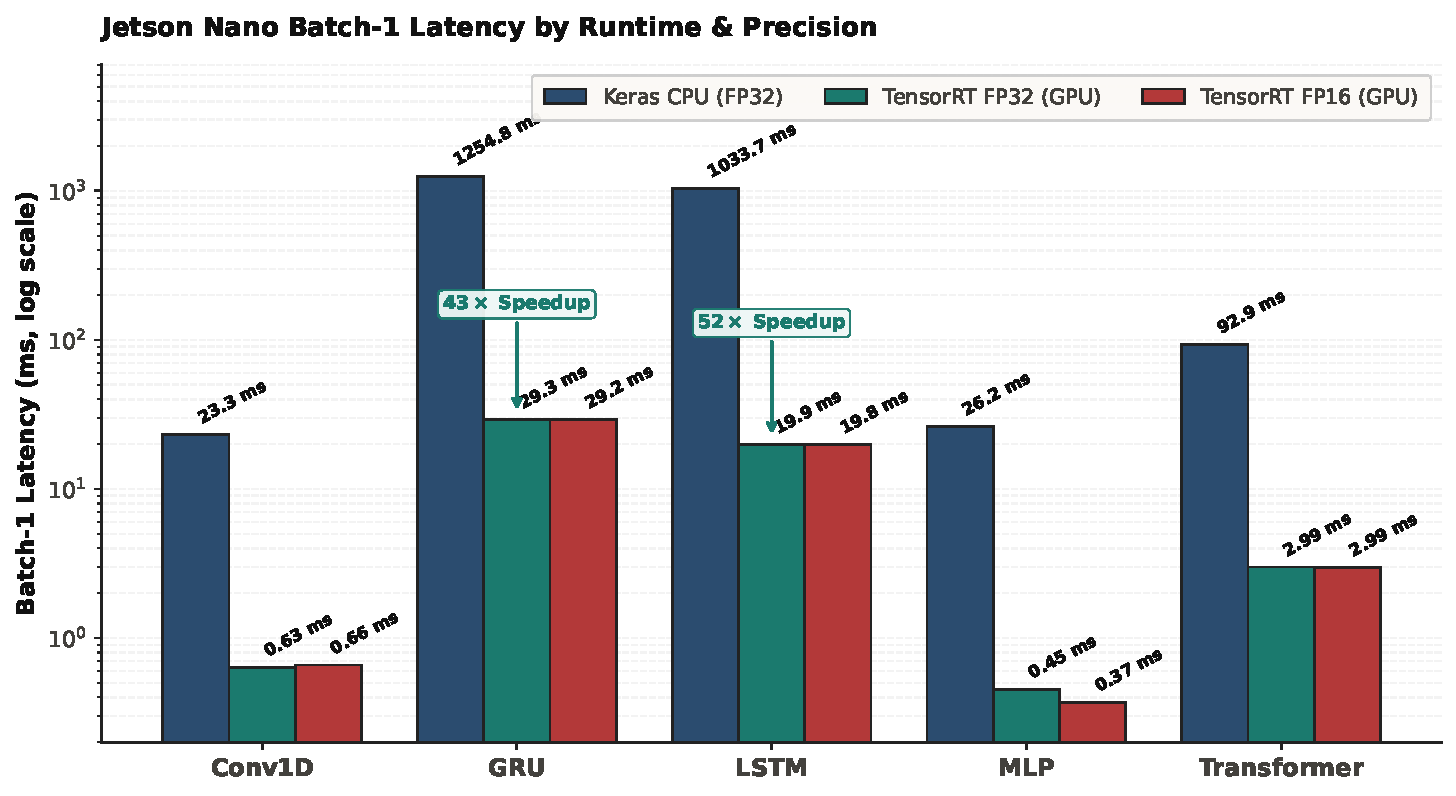
\includegraphics[width=0.92\textwidth]{jetson_latency_comparison.pdf}
\caption{Batch-1 inference latency comparison across host CPU (Keras FP32) and embedded GPU (TensorRT FP32 and FP16) runtimes.}
\label{fig:jetson-latency}
\end{figure}

\begin{figure}[t]
\centering
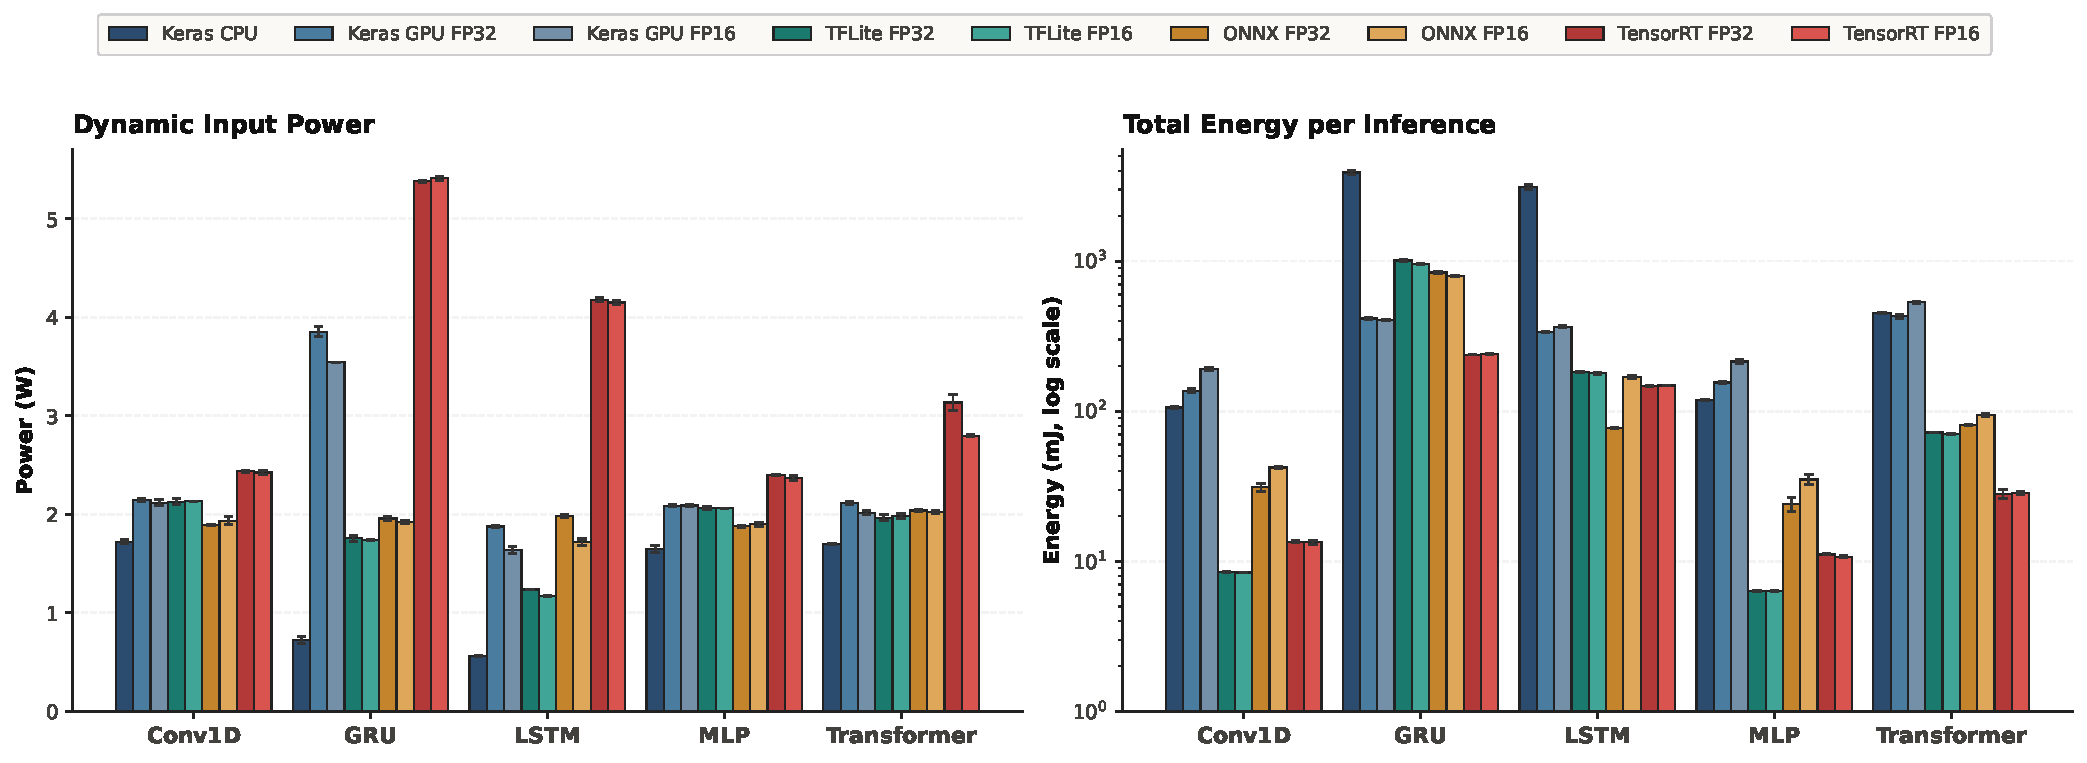
\includegraphics[width=0.95\textwidth]{jetson_power_energy.pdf}
\caption{Measured power and energy metrics on Jetson Nano: (left) dynamic module input power (W); (right) total energy per inference (mJ, $\log_{10}$ scale). Means and standard deviations over three isolated repetitions.}
\label{fig:jetson-power-energy}
\end{figure}

\begin{figure}[t]
\centering
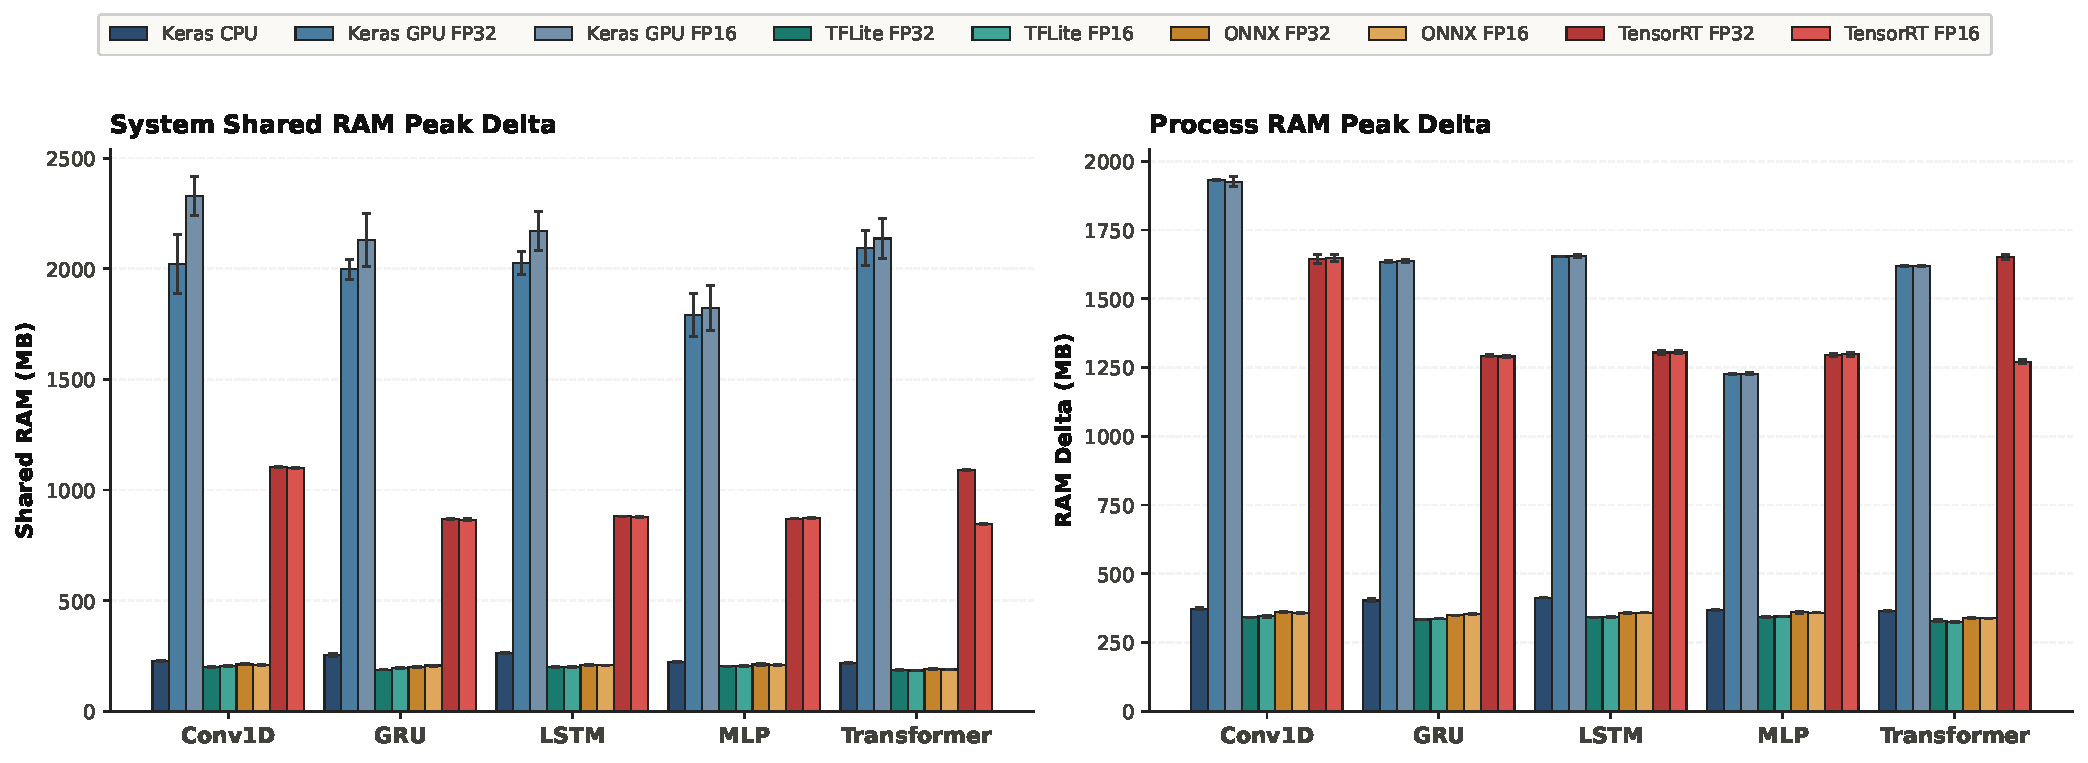
\includegraphics[width=0.95\textwidth]{jetson_memory_footprint.pdf}
\caption{Unified memory footprint allocation on Jetson Nano: (left) system shared RAM active peak delta (MB) from system telemetry; (right) process peak RSS delta (MB) from process status telemetry. GPU TensorRT context adds $\sim$845--1{,}100~MB system RAM vs $\sim$185--212~MB for CPU runtimes (Table~\ref{tab:selected-results}).}
\label{fig:jetson-memory-footprint}
\end{figure}

\begin{figure}[t]
\centering
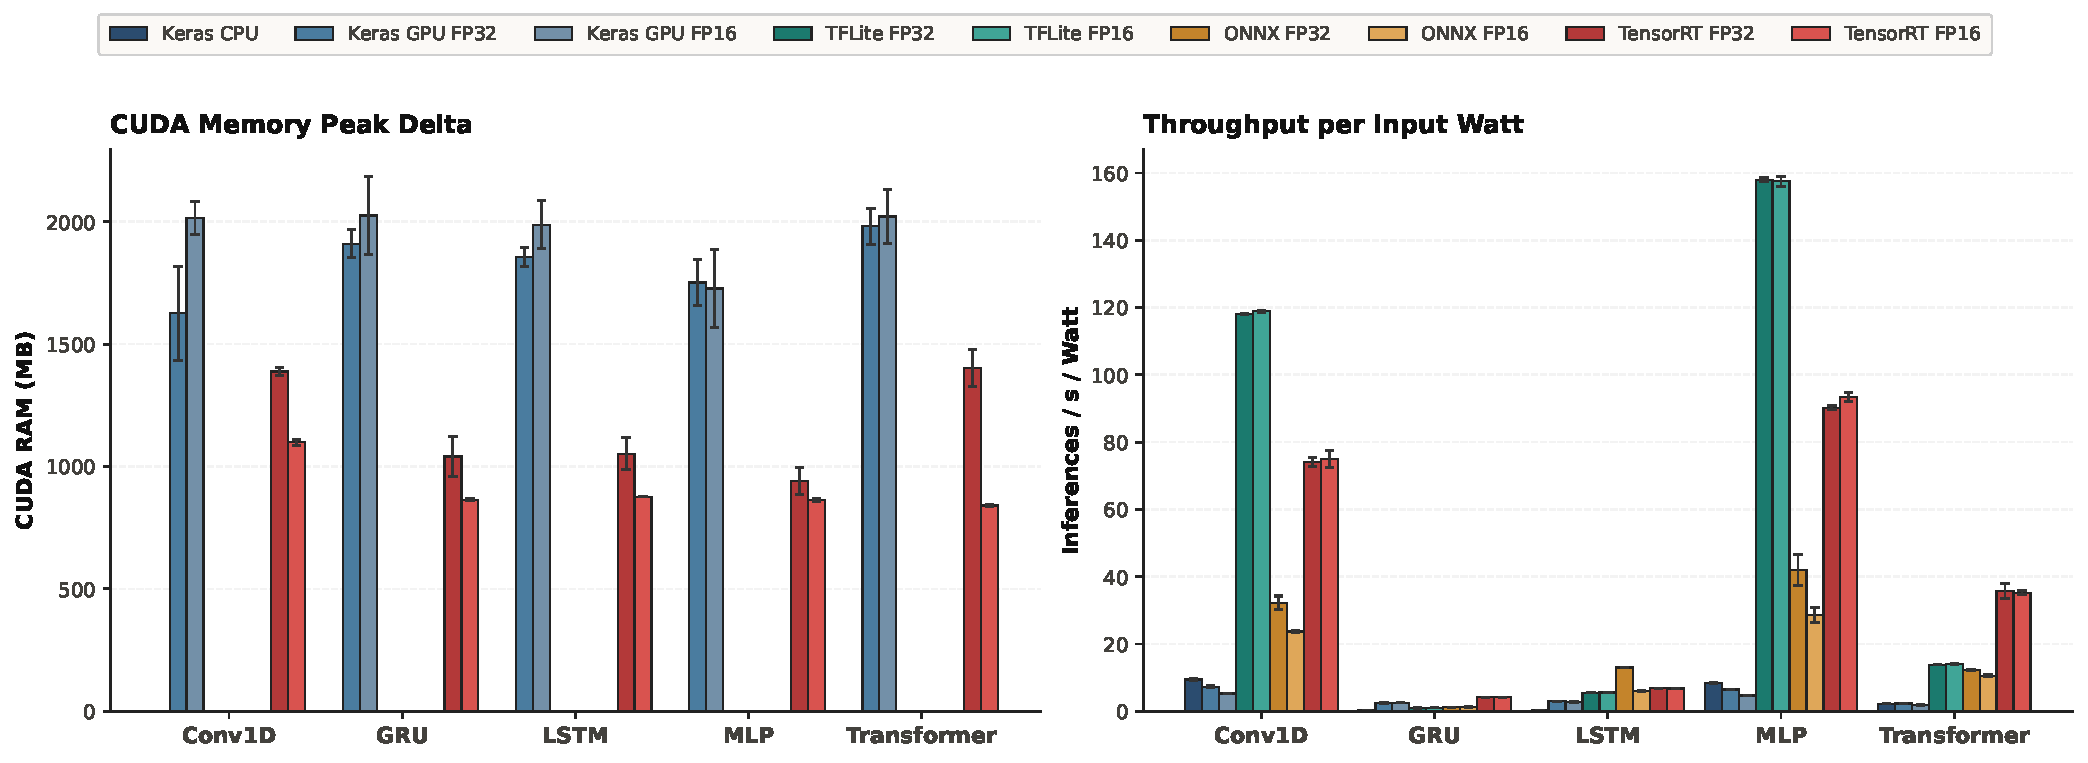
\includegraphics[width=0.95\textwidth]{jetson_efficiency_throughput.pdf}
\caption{GPU context allocation and computational energy efficiency on Jetson Nano: (left) CUDA memory allocation peak delta (MB); (right) sustained throughput per input Watt (inferences/s/W).}
\label{fig:jetson-efficiency-throughput}
\end{figure}

\begin{figure}[t]
\centering
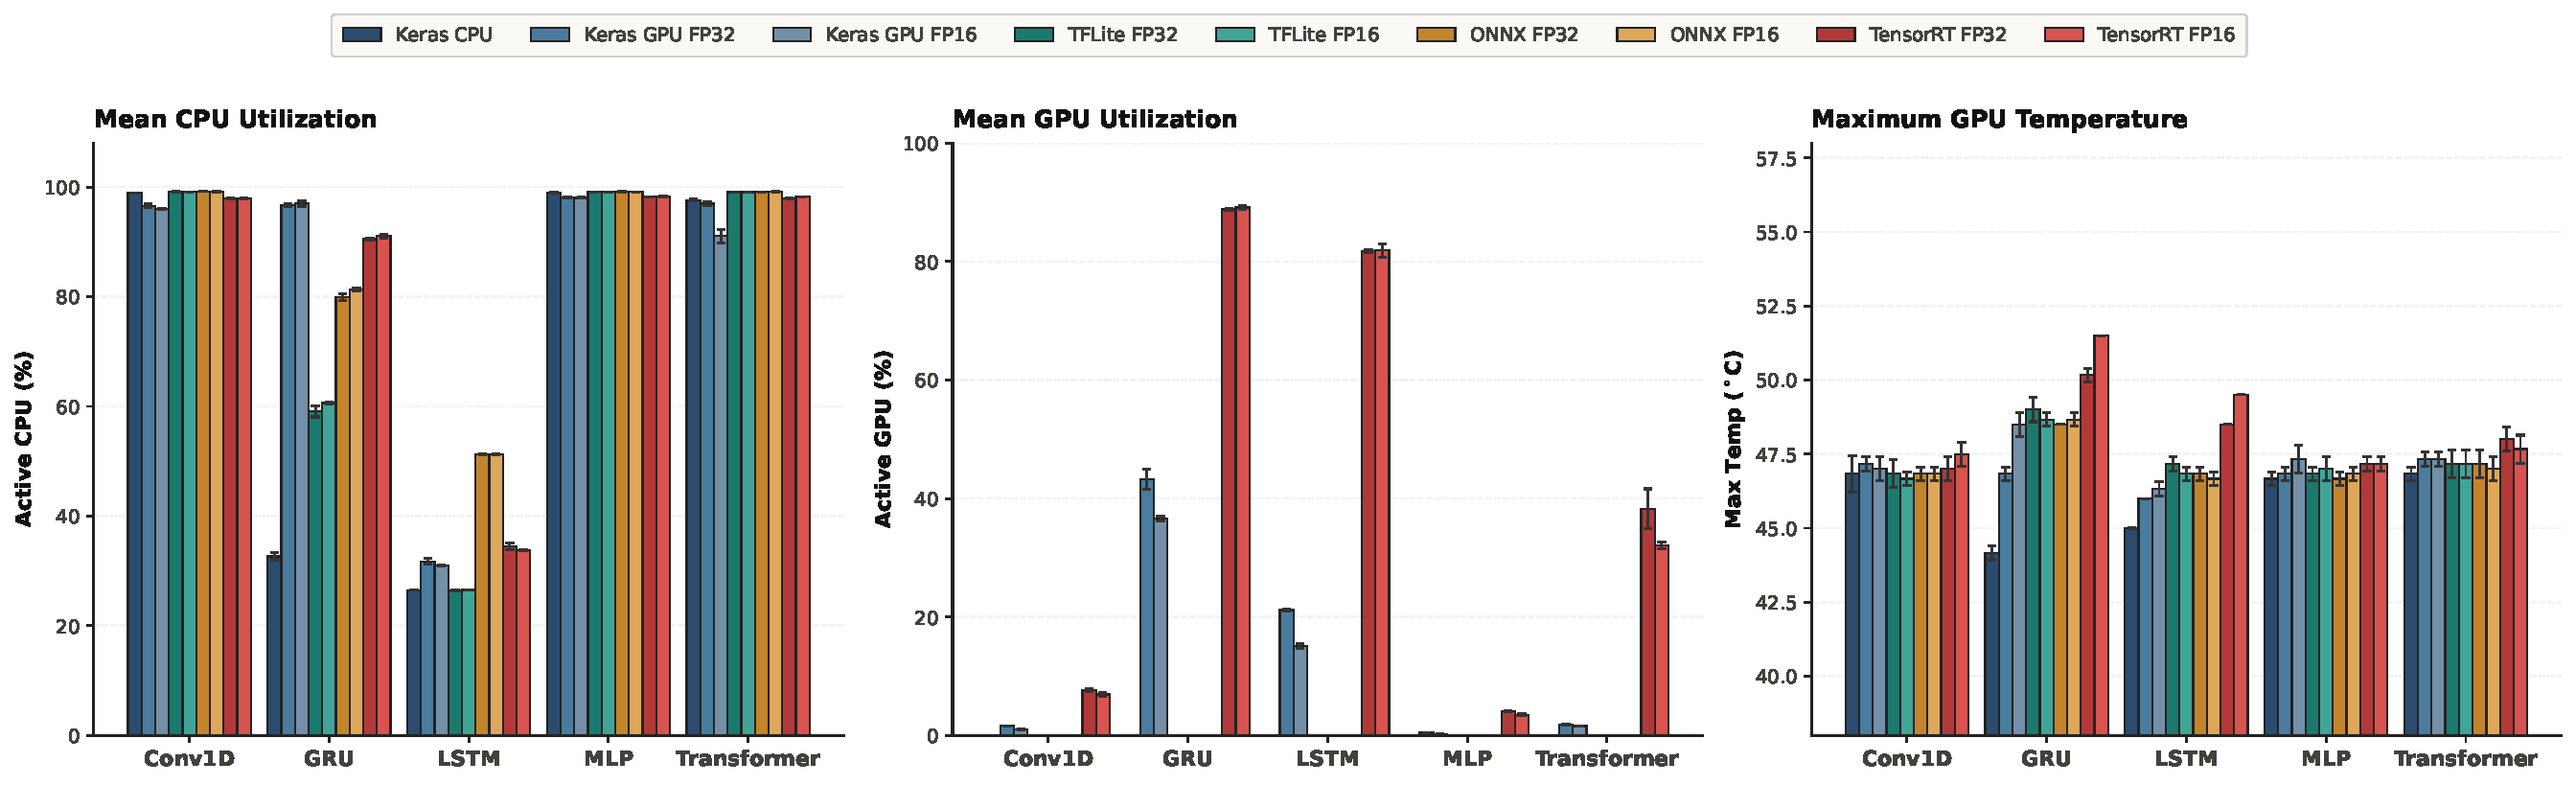
\includegraphics[width=0.95\textwidth]{jetson_utilization_thermal.pdf}
\caption{Mean CPU/GPU utilization and maximum GPU temperature during matched 15-s sustained inference windows.}
\label{fig:jetson-utilization-thermal}
\end{figure}

\begin{figure}[t]
\centering
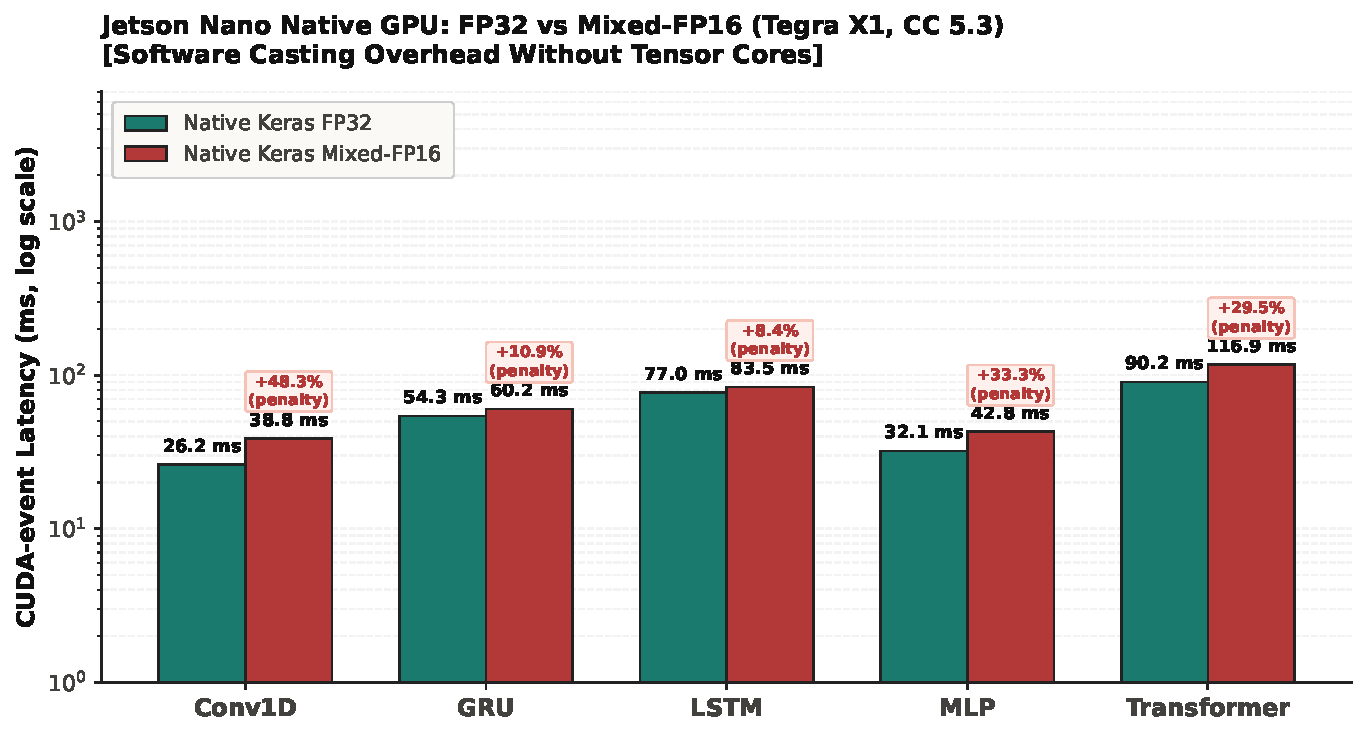
\includegraphics[width=0.82\textwidth]{native_gpu_precision_comparison.pdf}
\caption{Native TensorFlow GPU FP32 versus mixed-FP16~\cite{micikevicius2018mixed} evaluation latency on Jetson Nano (CUDA events, $\log_{10}$ scale). Mixed FP16 is $8.4\%$--$48.3\%$ slower across all five architectures on the Maxwell GPU on the evaluated hardware.}
\label{fig:native-gpu-precision}
\end{figure}

\subsection{Resource and Hardware Behavior}
Figs.~\ref{fig:jetson-latency}--\ref{fig:native-gpu-precision} present the comprehensive hardware profiling results:
\begin{itemize}
    \item \textbf{Memory Footprint:} CPU runtimes (TFLite, ONNX) maintain small system RAM footprints ($\approx 185$--$212\text{ MB}$ delta). GPU execution in TensorRT instantiates an internal CUDA driver runtime context, requiring 845--1,098 MB of system memory (Fig.~\ref{fig:jetson-memory-footprint}).
    \item \textbf{Native GPU Mixed Precision Inefficiency:} As shown in Fig.~\ref{fig:native-gpu-precision}, native Keras GPU mixed FP16~\cite{micikevicius2018mixed} is consistently slower than native FP32 across all architectures (e.g., 38.80 ms vs 26.17 ms for Conv1D, 116.86 ms vs 90.24 ms for Transformer). The Maxwell GPU lacks Tensor Cores. The benchmark does not separately time precision conversions and arithmetic kernels.
    \item \textbf{Thermal and Utilization Characteristics:} Sustained TensorRT inference for GRU drives GPU utilization to 89.1\% and power to 7.88 W, increasing GPU core temperature to $51.5^\circ\text{C}$ (Fig.~\ref{fig:jetson-utilization-thermal}), during the 15-s profiling window.
\end{itemize}

\section{Discussion}
\label{sec:discussion}

The experimental findings challenge common preconceptions regarding edge model optimization, with implications for heterogeneous supercomputing at the edge:
\begin{enumerate}
    \item \textbf{The Myth of Universal Quantization Speedup:} Lower precision is not universally beneficial on embedded SoCs. On the Maxwell GPU, TensorRT FP16 matches rather than exceeds FP32 latency (GRU: 29.20~ms vs 29.31~ms) due to the absence of Tensor Core matrix acceleration, serving primarily to reduce serialized engine memory footprint (e.g., Transformer 1402~MB$\to$841~MB CUDA). On CPU, ONNX FP16 is slower than ONNX FP32 due to software half-precision emulation overhead.
    \item \textbf{Architecture-Specific Operator Wins:} Model architecture dominates execution latency more than bit precision. TensorRT delivers extraordinary gains for recurrent models ($43\times$--$52\times$), transforming unusable CPU models into deployable edge detectors. For feedforward models (MLP, Conv1D), lightweight CPU runtimes (TFLite) outpace TensorRT by avoiding CUDA launch overhead --- a classic host-accelerator dispatch trade-off relevant to supercomputing task mapping.
    \item \textbf{Fidelity Validation is Essential:} Had this benchmark evaluated models solely by execution latency or tensor MSE, Transformer TensorRT FP16 and LSTM TFLite FP32 would appear optimal. Downstream decision validation exposes that both configurations corrupt classification boundaries, analogous to silent data corruption in HPC --- a hardware-reliability concern.
    \item \textbf{Portability across accelerator generations.} The measurements characterize the Jetson Nano with the reported software stack. A separate campaign is needed to evaluate integer acceleration on newer SoCs and to test whether quantization-aware training improves agreement with the FP32 detector.
\end{enumerate}

\section{Conclusion, Systems Limitations, and Future Work}
\label{sec:conclusion}

This study benchmarked 60 attempted model--runtime--precision execution pathways (45 core FP32/FP16 plus 15 INT8) for self-supervised power converter anomaly detectors on the NVIDIA Jetson Nano. Implementing an end-to-end decision validation gate identified 37 validated and 8 fidelity-rejected core configurations; all 15 INT8 configurations were non-deployable. INT8 was systematically analyzed and excluded due to Maxwell hardware limitations, ONNX parser QDQ rejections, and decision corruption. 

The optimal validated operating point is MLP in TensorFlow Lite FP32, achieving 0.168 ms latency, 710.15 inferences/s, and 2.91 mJ dynamic energy per inference. For recurrent architectures, TensorRT FP16 enables practical deployment with $43\times$--$52\times$ latency reductions, and only the evaluated FP32 Transformer paths pass the decision-agreement criterion.

\subsection{Systems-Level Limitations and Future Research Trajectories}
While this work establishes rigorous benchmarking and fidelity-gating protocols, three key systems-level limitations define the future research agenda:
\begin{enumerate}
    \item \textbf{Hardware Generational Bound (Maxwell vs. Modern Edge Accelerators):} The Maxwell Tegra X1 testbed lacks hardware integer dot-product units (DP4A) and Tensor Cores. Future research will benchmark modern edge SoCs (e.g., NVIDIA Jetson Orin Nano / Orin NX with Ampere CC 8.7) and evaluate whether Quantization-Aware Training (QAT) with Learnable Step Size Quantization (LSQ) can adaptively preserve the narrow metric separation around threshold $\gamma$, unlocking low-power integer acceleration without decision flips.
    \item \textbf{Neural Backbone vs. End-to-End Signal Chain Integration:} The present study times neural forward propagation and evaluates detector decision agreement. A complete production edge instrument requires integrating front-end analog-to-digital converter (ADC) DMA streaming, hardware FFT/chirp excitation generation, and flash memory wear-leveling into a unified bare-metal or real-time operating system (RTOS) firmware architecture.
    \item \textbf{Dynamic Environmental Drift (Thermal and Voltage Variations):} The decision threshold $\gamma$ is calibrated under static temperature and input voltage conditions. In industrial field deployments, ambient temperature fluctuations ($ -40^\circ\text{C}$ to $+85^\circ\text{C}$) and wide input voltage variations shift nominal baseline responses. Future work will investigate adaptive online threshold compensation algorithms that dynamically track thermal and electrical operating points without retraining.
\end{enumerate}

\section{Reproducibility Statement}
\label{sec:reproducibility}

The \href{https://github.com/igmsalinas/fault-converters-code/tree/9e13ccdd263346e2eadd15102fe096393a64d38a}{code repository} contains the model export, timing, power telemetry, and fidelity validation tools. The \href{https://github.com/igmsalinas/fault-converters-data/tree/4950ecf604fab8b63395201b2d4a28af88fae8e8}{data repository} contains archived model artifacts, engine files, benchmark reports, and archived test scores for the fixed-load campaign.

\section*{Data Availability Statement}
Access to the archives requires repository permissions. Large artifacts are stored using Git LFS. Recreating the hardware measurements requires a compatible Jetson Nano software and hardware environment. The fixed-load raw cohort remains to be archived.

\section*{Conflict of Interest Statement}
The authors declare no competing financial or non-financial interests.

\bibliographystyle{IEEEtran}
\bibliography{references}

\end{document}
